% Options for packages loaded elsewhere
\PassOptionsToPackage{unicode}{hyperref}
\PassOptionsToPackage{hyphens}{url}
\PassOptionsToPackage{dvipsnames,svgnames,x11names}{xcolor}
%
\documentclass[
  a4paper,
  DIV=11,
  numbers=noendperiod]{scrartcl}

\usepackage{amsmath,amssymb}
\usepackage{iftex}
\ifPDFTeX
  \usepackage[T1]{fontenc}
  \usepackage[utf8]{inputenc}
  \usepackage{textcomp} % provide euro and other symbols
\else % if luatex or xetex
  \usepackage{unicode-math}
  \defaultfontfeatures{Scale=MatchLowercase}
  \defaultfontfeatures[\rmfamily]{Ligatures=TeX,Scale=1}
\fi
\usepackage{lmodern}
\ifPDFTeX\else  
    % xetex/luatex font selection
\fi
% Use upquote if available, for straight quotes in verbatim environments
\IfFileExists{upquote.sty}{\usepackage{upquote}}{}
\IfFileExists{microtype.sty}{% use microtype if available
  \usepackage[]{microtype}
  \UseMicrotypeSet[protrusion]{basicmath} % disable protrusion for tt fonts
}{}
\makeatletter
\@ifundefined{KOMAClassName}{% if non-KOMA class
  \IfFileExists{parskip.sty}{%
    \usepackage{parskip}
  }{% else
    \setlength{\parindent}{0pt}
    \setlength{\parskip}{6pt plus 2pt minus 1pt}}
}{% if KOMA class
  \KOMAoptions{parskip=half}}
\makeatother
\usepackage{xcolor}
\setlength{\emergencystretch}{3em} % prevent overfull lines
\setcounter{secnumdepth}{5}
% Make \paragraph and \subparagraph free-standing
\ifx\paragraph\undefined\else
  \let\oldparagraph\paragraph
  \renewcommand{\paragraph}[1]{\oldparagraph{#1}\mbox{}}
\fi
\ifx\subparagraph\undefined\else
  \let\oldsubparagraph\subparagraph
  \renewcommand{\subparagraph}[1]{\oldsubparagraph{#1}\mbox{}}
\fi


\providecommand{\tightlist}{%
  \setlength{\itemsep}{0pt}\setlength{\parskip}{0pt}}\usepackage{longtable,booktabs,array}
\usepackage{calc} % for calculating minipage widths
% Correct order of tables after \paragraph or \subparagraph
\usepackage{etoolbox}
\makeatletter
\patchcmd\longtable{\par}{\if@noskipsec\mbox{}\fi\par}{}{}
\makeatother
% Allow footnotes in longtable head/foot
\IfFileExists{footnotehyper.sty}{\usepackage{footnotehyper}}{\usepackage{footnote}}
\makesavenoteenv{longtable}
\usepackage{graphicx}
\makeatletter
\def\maxwidth{\ifdim\Gin@nat@width>\linewidth\linewidth\else\Gin@nat@width\fi}
\def\maxheight{\ifdim\Gin@nat@height>\textheight\textheight\else\Gin@nat@height\fi}
\makeatother
% Scale images if necessary, so that they will not overflow the page
% margins by default, and it is still possible to overwrite the defaults
% using explicit options in \includegraphics[width, height, ...]{}
\setkeys{Gin}{width=\maxwidth,height=\maxheight,keepaspectratio}
% Set default figure placement to htbp
\makeatletter
\def\fps@figure{htbp}
\makeatother
\newlength{\cslhangindent}
\setlength{\cslhangindent}{1.5em}
\newlength{\csllabelwidth}
\setlength{\csllabelwidth}{3em}
\newlength{\cslentryspacingunit} % times entry-spacing
\setlength{\cslentryspacingunit}{\parskip}
\newenvironment{CSLReferences}[2] % #1 hanging-ident, #2 entry spacing
 {% don't indent paragraphs
  \setlength{\parindent}{0pt}
  % turn on hanging indent if param 1 is 1
  \ifodd #1
  \let\oldpar\par
  \def\par{\hangindent=\cslhangindent\oldpar}
  \fi
  % set entry spacing
  \setlength{\parskip}{#2\cslentryspacingunit}
 }%
 {}
\usepackage{calc}
\newcommand{\CSLBlock}[1]{#1\hfill\break}
\newcommand{\CSLLeftMargin}[1]{\parbox[t]{\csllabelwidth}{#1}}
\newcommand{\CSLRightInline}[1]{\parbox[t]{\linewidth - \csllabelwidth}{#1}\break}
\newcommand{\CSLIndent}[1]{\hspace{\cslhangindent}#1}

\usepackage{booktabs}
\usepackage{longtable}
\usepackage{array}
\usepackage{multirow}
\usepackage{wrapfig}
\usepackage{float}
\usepackage{colortbl}
\usepackage{pdflscape}
\usepackage{tabu}
\usepackage{threeparttable}
\usepackage{threeparttablex}
\usepackage[normalem]{ulem}
\usepackage{makecell}
\usepackage{xcolor}
\KOMAoption{captions}{tableheading}
\makeatletter
\makeatother
\makeatletter
\makeatother
\makeatletter
\@ifpackageloaded{caption}{}{\usepackage{caption}}
\AtBeginDocument{%
\ifdefined\contentsname
  \renewcommand*\contentsname{Table of contents}
\else
  \newcommand\contentsname{Table of contents}
\fi
\ifdefined\listfigurename
  \renewcommand*\listfigurename{List of Figures}
\else
  \newcommand\listfigurename{List of Figures}
\fi
\ifdefined\listtablename
  \renewcommand*\listtablename{List of Tables}
\else
  \newcommand\listtablename{List of Tables}
\fi
\ifdefined\figurename
  \renewcommand*\figurename{Figure}
\else
  \newcommand\figurename{Figure}
\fi
\ifdefined\tablename
  \renewcommand*\tablename{Table}
\else
  \newcommand\tablename{Table}
\fi
}
\@ifpackageloaded{float}{}{\usepackage{float}}
\floatstyle{ruled}
\@ifundefined{c@chapter}{\newfloat{codelisting}{h}{lop}}{\newfloat{codelisting}{h}{lop}[chapter]}
\floatname{codelisting}{Listing}
\newcommand*\listoflistings{\listof{codelisting}{List of Listings}}
\makeatother
\makeatletter
\@ifpackageloaded{caption}{}{\usepackage{caption}}
\@ifpackageloaded{subcaption}{}{\usepackage{subcaption}}
\makeatother
\makeatletter
\@ifpackageloaded{tcolorbox}{}{\usepackage[skins,breakable]{tcolorbox}}
\makeatother
\makeatletter
\@ifundefined{shadecolor}{\definecolor{shadecolor}{rgb}{.97, .97, .97}}
\makeatother
\makeatletter
\makeatother
\makeatletter
\makeatother
\ifLuaTeX
  \usepackage{selnolig}  % disable illegal ligatures
\fi
\IfFileExists{bookmark.sty}{\usepackage{bookmark}}{\usepackage{hyperref}}
\IfFileExists{xurl.sty}{\usepackage{xurl}}{} % add URL line breaks if available
\urlstyle{same} % disable monospaced font for URLs
\hypersetup{
  pdftitle={Assignment 1: Data and Descriptive},
  pdfauthor={Anine Therese Karlsen \& Mona Lisa Jones},
  colorlinks=true,
  linkcolor={blue},
  filecolor={Maroon},
  citecolor={Blue},
  urlcolor={Blue},
  pdfcreator={LaTeX via pandoc}}

\title{Assignment 1: Data and Descriptive}
\author{Anine Therese Karlsen \& Mona Lisa Jones}
\date{}

\begin{document}
\maketitle
\begin{abstract}
This assignment aims to acquire, process, and analyze sub-national GDP
and population data for a subset of European countries. Calculate GDP
per capita and explore regional inequity using various descriptive
statistics and visualizations.
\end{abstract}
\ifdefined\Shaded\renewenvironment{Shaded}{\begin{tcolorbox}[sharp corners, interior hidden, frame hidden, borderline west={3pt}{0pt}{shadecolor}, boxrule=0pt, enhanced, breakable]}{\end{tcolorbox}}\fi

\hypertarget{introduction}{%
\section{Introduction}\label{introduction}}

While national GDP and GDP per capita are vital indicators of a
country's aggregate economic health, they do not shed light on how
wealth or income is distributed among its residents. A high national GDP
can, paradoxically, coexist with pockets of regional deprivation
(Lessmann and Seidel 2017).

The truth of this statement becomes more evident when taking a closer
look in to into sub-national data. Regional wealth disparities are of
prime concern, especially when crafting policies for equitable growth
(Lessmann and Seidel 2017). A country's macro-level prosperity does not
automatically guarantee that all its regions partake equally in this
wealth. By studying smaller regions within a country, it is possible to
get a more nuanced narrative about the state of regional economic
disparities (Lessmann and Seidel 2017).

This assignment is anchored in this very premise. It seeks to acquire,
process, and analyse sub-national GDP and population data for a selected
subset of European countries, namely France, Denmark, Hungary, Portugal,
and Slovakia, spanning the period from 2000 to 2020. The overarching aim
is to calculate GDP per capita for these regions and delve into the
intricacies of regional inequity. This exploration will be underpinned
by various descriptive statistics, visualizations, and analytical
techniques to paint a comprehensive picture of regional economic
landscapes.

Using time series data observing the GDP per capita and GINI trends
across regions and over time, we can discern whether certain areas are
ahead or behind in economic performance.

\hypertarget{literature-review}{%
\section{Literature review}\label{literature-review}}

``In recent decades, the regional distribution of incomes within
countries has attracted considerable interest among academics and policy
makers.'' (Lessmann and Seidel 2017)

Slovakia, experienced significant economic growth. Their GDP per capita
grew faster than the older EU member states, albeit from a lower
starting point, leading to a convergence ({``Full Article: The Causal
Impact of Economic Growth on Material Use in Europe,''} n.d.).

The global financial crisis and subsequent European debt crisis had
significant impacts on European economies. GDP per capita declined in
several countries, particularly those hit hardest by the crisis, such as
Greece, Spain, and Portugal. Some regions took many years to recover to
pre-crisis levels, while others, especially in Northern Europe,
recovered more quickly (Lewis and Verhoeven, n.d.).

Major metropolitan areas, like Paris in France, London in the UK, and
Berlin in Germany, often grew faster than other regions in their
respective countries, leading to increasing spatial disparities (Kiuru
and Inkinen 2019).

Denmark maintained relatively high levels of GDP per capita throughout
this period, benefiting from a diversified economy, strong institutions,
and a high degree of economic openness. It did face challenges during
the 2008 economic crisis but recovered relatively quickly ({``Dynamics
of Technological Innovation, Energy Consumption, Energy Price and
Economic Growth in Denmark - Murad - 2019 - Environmental Progress \&
Sustainable Energy - Wiley Online Library,''} n.d.).

Slovenia, which joined the EU in 2004, showed growth in GDP per capita,
though it too was affected by the global economic downturn in 2008.
However, it managed to recover in the subsequent years ({``Full Article:
The Causal Impact of Economic Growth on Material Use in Europe,''}
n.d.).

Regional disparities persisted, with the Île-de-France region (which
includes Paris) significantly outperforming other regions in terms of
GDP per capita. The gap between urban and rural areas also remained a
topic of discussion ({``Regional Inequality in Europe: Evidence, Theory
and Policy Implications \textbar{} Journal of Economic Geography
\textbar{} Oxford Academic,''} n.d.).

Towards the end of this period, in early 2020, the COVID-19 pandemic
posed a new set of challenges for European economies, causing
significant contractions in GDP per capita across many regions
({``Regional Inequality in Europe: Evidence, Theory and Policy
Implications \textbar{} Journal of Economic Geography \textbar{} Oxford
Academic,''} n.d.).

\hypertarget{part-a-sub-national-gdp-and-gdp-per-capita}{%
\section{Part A: Sub-national GDP and GDP per
Capita}\label{part-a-sub-national-gdp-and-gdp-per-capita}}

\hypertarget{data-acquisition-and-datasets}{%
\subsection{Data Acquisition and
datasets}\label{data-acquisition-and-datasets}}

The first thing we did in this assignment was to acquire our data.
Trough Eurostat, we could download the datasets nama\_10r\_3gdp and
demo\_r\_pjanggr3 as csv files, as well as filter the data by our
preferences before downloading it. As per the assignment, we filtered
the dataset by choosing the years 2000 to 2020. Furthermore, we selected
the NUTS 3 region for the nations we were given, which were Portugal,
France, Hungary, Slovakia and Denmark. Finally, we specified the data to
be in million Euro.

\hypertarget{gdp-nama_10r_3gdp}{%
\subsubsection{GDP (nama\_10r\_3gdp)}\label{gdp-nama_10r_3gdp}}

The nama\_10r\_3gdp dataset from Eurostat provides insights into GDP at
regional level using the NUTS classification system. It furnishes GDP
values in both current prices and adjusted for inflation, with some
figures given in purchasing power standards (PPS) to account for price
level differences between countries. The data is often structured by
year and region Eurostat (2023a).

The GDP at market prices represents the final result of production
activities of resident producer units within a region or nation. It is
calculated as the sum of the gross value added across various
institutional sectors or industries, augmented by taxes and reduced by
subsidies on products (which are not allocated to specific sectors or
industries). This also balances out in the total economy production
account. In terms of methodology, while national accounts compile GDP
from the expenditure side, regional accounts don't adopt this approach
due to the complexities of accurately mapping inter-regional flows of
goods and services.

The different measures for the regional GDP are absolute figures in €
and Purchasing Power Standards (PPS), figures per inhabitant and
relative data compared to the EU Member States average Eurostat (2023b).

\hypertarget{population-demo_r_pjanggr3}{%
\subsubsection{Population
(demo\_r\_pjanggr3)}\label{population-demo_r_pjanggr3}}

Using the NUTS categorization once more, Eurostat's demo\_r\_pjanggr3
records annual population changes at the regional level. This dataset
includes information on births, deaths, net migration, and may also
include demographic information on age and gender. It's also often
displayed in a year-by-region format, and the data usually spans in
yearly intervals Eurostat (2023c).

Eurostat's primary source for yearly demographic data at the regional
level stems from the Unified Demography (Unidemo) project. The project
covers 37 countries and is the central repository for demographic and
migration-related data. Specific metrics gathered under UNIDEMO
encompass population counts at the close of the calendar year and events
such as births and deaths occurring within that year. Additionally, data
on marriages, divorces, and migration flows are recorded.

For the purpose of this research, the demographic data references the
NUTS 2016 classification, which provides a detailed breakdown of the
European Union's territory Eurostat (2021).

\hypertarget{nuts-classification}{%
\subsubsection{NUTS classification}\label{nuts-classification}}

The Nomenclature of Territorial Units for Statistics (NUTS) offers a
stratified system to segment the economic territory of the EU (including
the UK) to facilitate the consistent collection and harmonization of
regional statistics across Europe. The NUTS regions range from NUTS 0
Country level to NUTS 3 small units such as municipalities level. ~

\hypertarget{gdp-per-capita-calculation}{%
\subsection{GDP per Capita
Calculation}\label{gdp-per-capita-calculation}}

The formula for calculating GDP per Capita is as follows:

\(y_i=GDP_i/population_i\)

After calculating the GDP per capita for all NUTS 3 regions in our
assigned countries, we can see that there is a large spread between the
figures for the various regions. In this assignement we want to look at
regional inequity; in order to do this in a valuable way we have to
divide between the different countries. By doing this, we can gain
important insights on regional differences that we can utilize, for
instance, to discuss national policy on equity and sustainable economic
development in regions.

\hypertarget{descriptive-statistics}{%
\subsubsection{Descriptive statistics}\label{descriptive-statistics}}

In this part we will report and interpret different types of essential
descriptive statistics. Measuring regional income inequality is
challenging due to heterogeneity of regions. The number of regions in
our data set varies largely in size and population. Since the focus of
this paper is purely growth and changes in inequities over time, the
variations of size and population density becomes a minor issue because
the country-level territorial heterogeneity is fixed.

``Interest in income inequality has led to the development of several
ways of measuring it. Two types of measures are of interest in this
paper----static and dynamic. \emph{Static measures} provide a snapshot
of these inequalities at a point of time whereas the dynamic
\emph{measures capture historical trends.}'' (læreboken)

In this part, we'll look at GDP per capita for our assigned countries on
a NUTS 3 level. In addition, we'll use different kinds of descriptive
statistics in order to further 0,37, is analyse this data. In this
analysis, we'll use Wooldridge (2020) for help.

By using figures, we can visualize the GDP per capita, and look at how
it varies among the different regions. In these figures, a line
represent one NUTS 3 region.

\textbf{Mean}

Calculate the mean to provide a representative value for a dataset,
facilitating understanding of its central tendency and serving as a
benchmark against which deviations and anomalies can be assessed, in
later steps when building and interpreting regression models.

\textbf{MMR}

A comparison of the GRDP (gross regional domestic product) per capita of
the region with the highest income to the region with the lowest income
(minimum per capita GRDP) provides a measure of the range of these
disparities. If this measure is small (close to 1), then it would mean
that the different regions have relatively equal incomes. If this
measure is large, then the interpretation is more problematic, as it
does not tell us if the high ratio is due to substantial variation in
the distribution of per capita GDRPs or the presence of outliers.
Nevertheless, maximum to minimum ratio (MMR) provides a quick, easy to
comprehend, and politically powerful measure of regional income
inequality.

\textbf{Standard diviation (SD)}

Calculating SD to quantify the dispersion or variability of a data set
around its mean. Helping us assess the degree of uncertainty,
variability, or risk associated with an economic variable or parameter,
which is crucial for understanding the reliability of estimations and
predictions (Wooldridge 2020).

\textbf{Median}

The median serves as a robust measure of central tendency, especially
when a dataset may have outliers or is skewed. Unlike the mean, the
median is not influenced by extreme values and, thus, can provide a
clearer picture of the ``typical'' value in situations where the data
distribution is not symmetrical (Wooldridge 2020).

\hypertarget{portugal}{%
\subsubsection{Portugal}\label{portugal}}

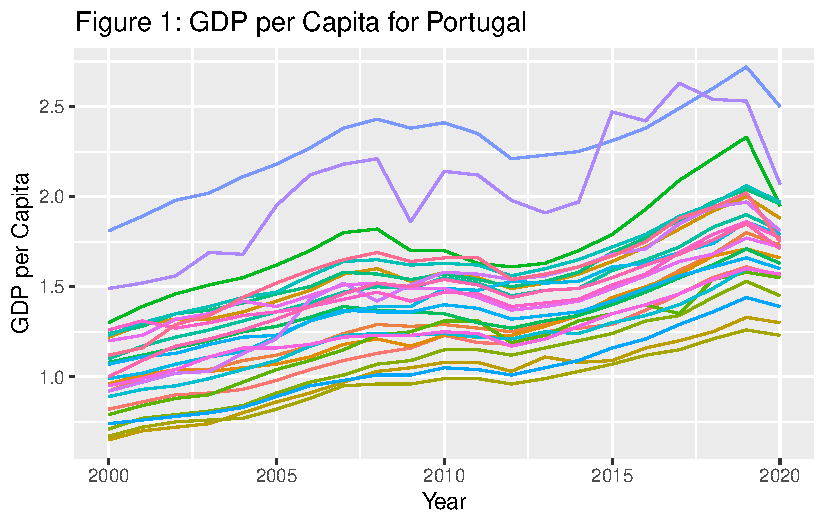
\includegraphics{assignment_1_files/figure-pdf/unnamed-chunk-7-1.pdf}

\begin{verbatim}
        GDP_per_capita
mean         1.4185524
median       1.3900000
std_dev      0.3702905
minimum      0.6500000
maximum      2.7200000
\end{verbatim}

By looking at figure for Portugal, we can see that the GDP per capita in
Portugal's regions appears to be fairly consistent. There is however
some regional variability. We can see that the regions around the big
cities like Lisbon have a higher GDP per capita compared to some more
rural areas. Since Lisbon is the capital of Portugal, there is probably
a higher concentration of industries, making it a economic center (which
again makes the GDP per capita higher).

To continue, we can see that the mean is a little higher that the
median, something that might indicate that regions like Lisbon are
pulling up the average. If we compare the standard derivation for
Portugal with the other countries, we'll see that is fairly low in
comparison. This might mean that there is not a lot of variability
between the GDP per capita across different regions in Portugal. The gap
between minimum and maximum is also low compared to other countries,
something that'll also show us that the economic disparity in Portugal
might not be as high as it is in other countries.

\hypertarget{france}{%
\subsubsection{France}\label{france}}

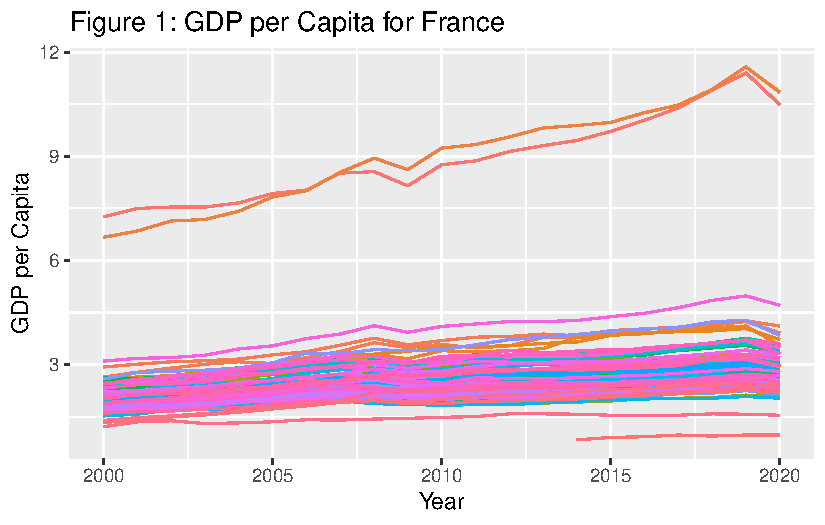
\includegraphics{assignment_1_files/figure-pdf/unnamed-chunk-10-1.pdf}

\begin{verbatim}
        GDP_per_capita
mean          2.630444
median        2.440000
std_dev       1.053767
minimum       0.830000
maximum      11.580000
\end{verbatim}

When looking at the figure for France, we can right away see that there
are some regions that have a much higher GDP per capita compared to the
other regions. The region that has the highest GDP per capita for all
years is the île-de-France region, one that also includes Paris. This
significant difference between the regions with the highest GDP per
capita and the lowest, shows us that there is a high concentration of
economic activity and wealth in a few urban regions. Similar to
Portugal, we can also again see that there is a difference between urban
and rural regions.

Just as in Portugal, there is also a higher mean in France as well.
Something that is different from the data in France compared to
Portugal, is that the standard derivation is higher, and the difference
between minimum and maximum is large. This strengthens what we have look
at earlier in the figure, with some regions having a high concentration
of wealth.

\hypertarget{hungary}{%
\subsubsection{Hungary}\label{hungary}}

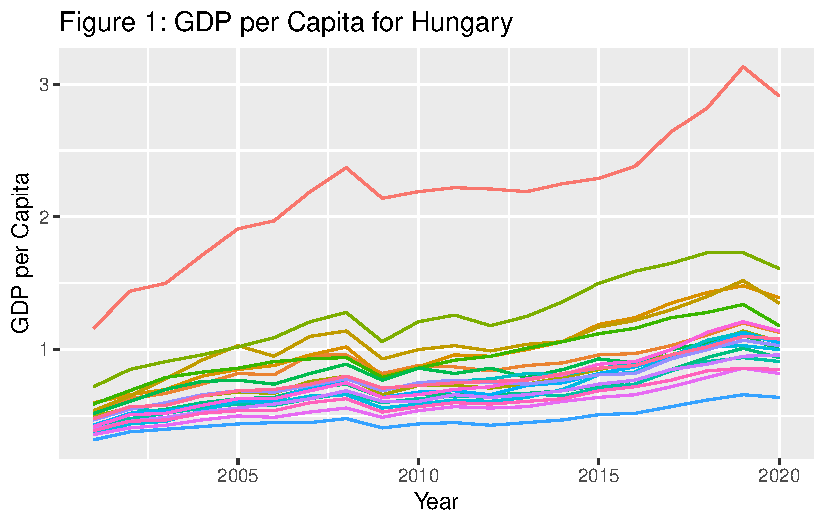
\includegraphics{assignment_1_files/figure-pdf/unnamed-chunk-13-1.pdf}

\begin{verbatim}
        GDP_per_capita
mean         0.8598000
median       0.7650000
std_dev      0.4059723
minimum      0.3200000
maximum      3.1300000
\end{verbatim}

In Hungary, most of the regions have similar GDP per Capita. One region
that sticks out by having a higher value, is the region of Budapest,
Hungary's biggest city.

We have here as well an mean that is larger than the median, high
standard derivation, and a large gap between minimum and maximum.

\hypertarget{slovakia}{%
\subsubsection{Slovakia}\label{slovakia}}

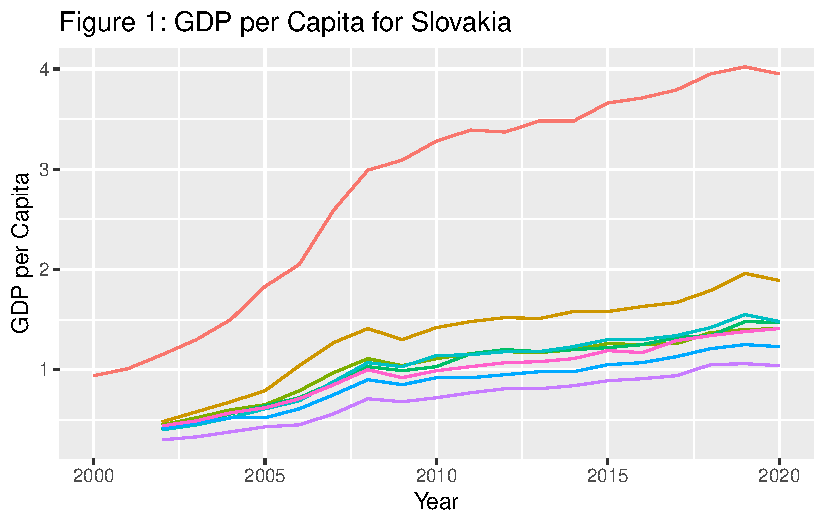
\includegraphics{assignment_1_files/figure-pdf/unnamed-chunk-16-1.pdf}

\begin{verbatim}
        GDP_per_capita
mean         1.2501948
median       1.0950000
std_dev      0.8018259
minimum      0.3000000
maximum      4.0200000
\end{verbatim}

In Slovakia as well, we have one region that has a much higher GDP per
capita than the rest of the regions. This region is Bratislava, which is
the biggest city and capital, something that might point to this city
being the economic capital of Slovakia as well.

Slovakia has also a mean higher that the median, and a large gap between
minimum and maximum. In addition, the standard derivation is pretty
high, meaning that there is some regions (or one region in this case)
that is far away from the rest of the regions when it comes to economic
development.

\hypertarget{denmark}{%
\subsubsection{Denmark}\label{denmark}}

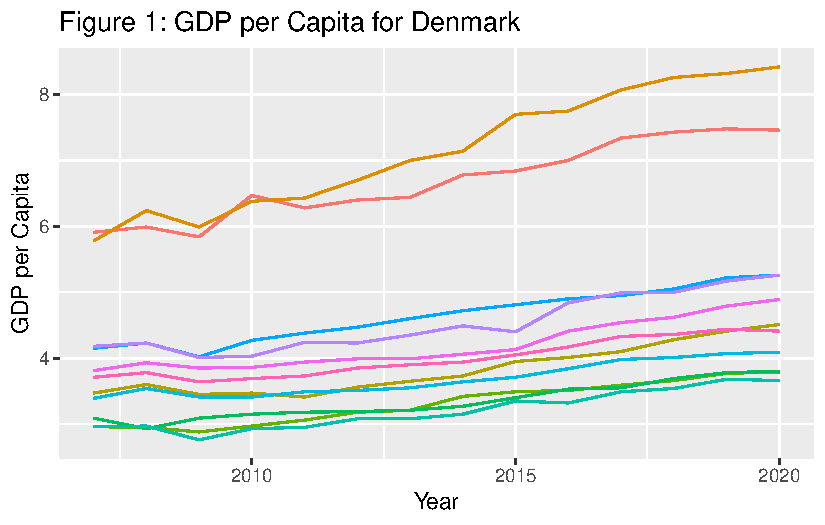
\includegraphics{assignment_1_files/figure-pdf/unnamed-chunk-19-1.pdf}

\begin{verbatim}
        GDP_per_capita
mean          4.419221
median        4.000000
std_dev       1.343933
minimum       2.760000
maximum       8.420000
\end{verbatim}

Lastly, we have Denmark. We can see similar pattern here as well, with
the capital Copenhagen being one of the regions with the highest GDP per
capita.

We can also see the same as the previous countries, with the mean being
higher than the median, which shows us that regions like Copenhagen
might drag the mean up by being much larger than the rest of the
regions.

\hypertarget{part-b-regional-inequity}{%
\section{Part B: Regional Inequity}\label{part-b-regional-inequity}}

\hypertarget{gini-coefficient-calculation}{%
\subsection{Gini Coefficient
Calculation}\label{gini-coefficient-calculation}}

With the use of the NUTS3 GDP per capita data and this formula:

\(GINW_j=\frac{1}{2 \bar{y_j}} \sum_{i}^{n_j}\sum_{l}^{n_j}\frac{p_i}{P_j} \frac{p_l}{P_j} |y_i-y_l|\)

we will compute the population-weighted GDP Gini coefficient for each
European NUTS2 region in our assigned countries.

The gini coefficient can help us measure inequality in a distribution,
as is therefore a useful tool for us to use when we look at regional
inequity. The closer the gini coefficient is to 1, the bigger the
inequality is; a number closer to 0 equals equality. When looking at the
gini coefficient for NUTS 2 regions, we also get a better overview over
differences in income between different regions, and it also makes it
easier to find the reasons as to why there is a difference between the
regions Hasell and Roser (2023).

After calculating the gini coefficients, we can see that there are some
similarities to the data we got from GDP per capita for NUTS 3 regions.
In order to see these similarities better, as well as look for other
important aspects that can be provided trough the calculations, we will
visualize the data in three different ways.

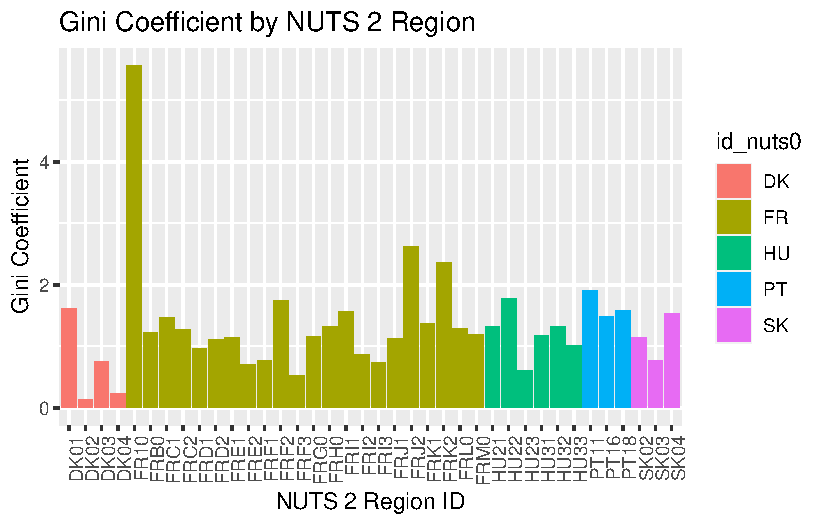
\includegraphics{assignment_1_files/figure-pdf/unnamed-chunk-23-1.pdf}

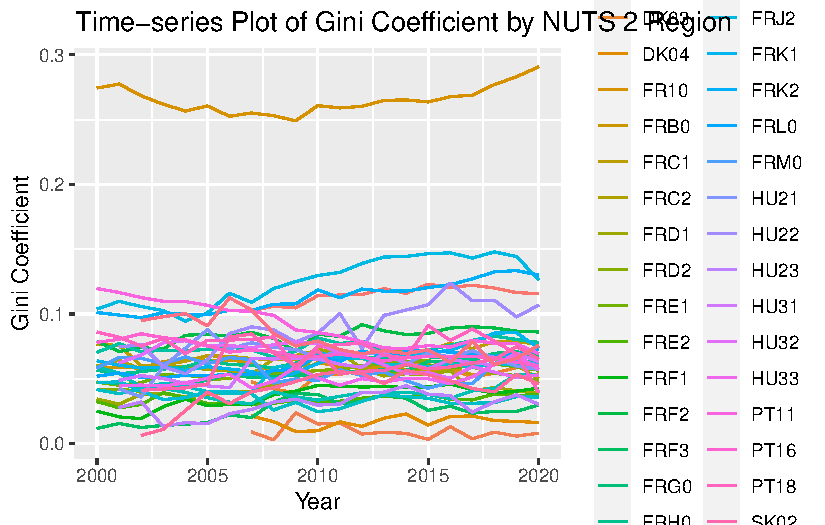
\includegraphics{assignment_1_files/figure-pdf/unnamed-chunk-24-1.pdf}

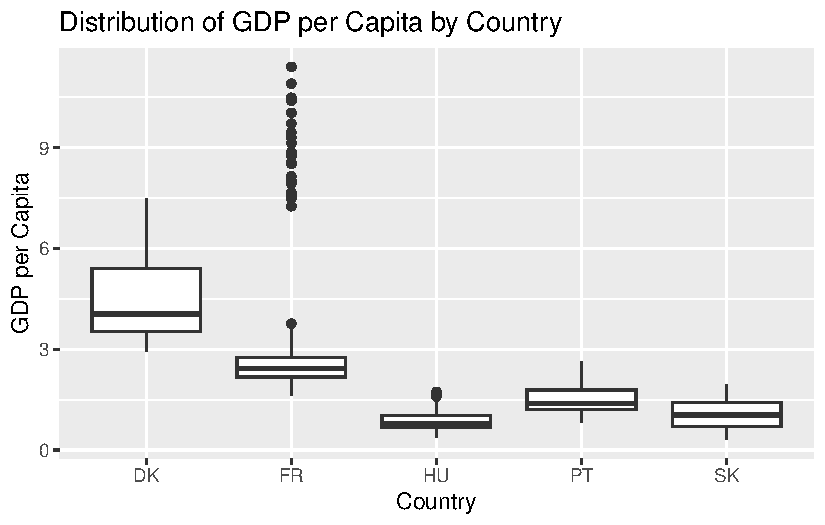
\includegraphics{assignment_1_files/figure-pdf/unnamed-chunk-25-1.pdf}

\hypertarget{discussion}{%
\subsection{Discussion}\label{discussion}}

\hypertarget{references}{%
\section*{References}\label{references}}
\addcontentsline{toc}{section}{References}

\hypertarget{refs}{}
\begin{CSLReferences}{1}{0}
\leavevmode\vadjust pre{\hypertarget{ref-dynamics}{}}%
{``Dynamics of Technological Innovation, Energy Consumption, Energy
Price and Economic Growth in Denmark - Murad - 2019 - Environmental
Progress \& Sustainable Energy - Wiley Online Library.''} n.d.
\url{https://aiche.onlinelibrary.wiley.com/doi/full/10.1002/ep.12905}.

\leavevmode\vadjust pre{\hypertarget{ref-eurostat2021}{}}%
Eurostat. 2021. {``Population Change - {Demographic} Balance and Crude
Rates at Regional Level ({NUTS} 3)~ (Demo\_r\_gind3).''}
https://ec.europa.eu/eurostat/cache/metadata/en/demo\_r\_gind3\_esms.htm.

\leavevmode\vadjust pre{\hypertarget{ref-eurostat2023}{}}%
---------. 2023a. {``Gross Domestic Product ({GDP}) at Current Market
Prices by {NUTS} 3 Regions.''}
https://ec.europa.eu/eurostat/databrowser/view/nama\_10r\_3gdp/default/table?lang=en.

\leavevmode\vadjust pre{\hypertarget{ref-eurostat2023c}{}}%
---------. 2023b. {``Regional Economic Accounts (Reg\_eco10).''}
https://ec.europa.eu/eurostat/cache/metadata/en/reg\_eco10\_esms.htm.

\leavevmode\vadjust pre{\hypertarget{ref-eurostat2023a}{}}%
---------. 2023c. {``Population on 1 {January} by Broad Age Group, Sex
and {NUTS} 3 Region.''}
https://ec.europa.eu/eurostat/databrowser/view/demo\_r\_pjanaggr3/default/table?lang=en.

\leavevmode\vadjust pre{\hypertarget{ref-fullart}{}}%
{``Full Article: The Causal Impact of Economic Growth on Material Use in
Europe.''} n.d.
\url{https://www.tandfonline.com/doi/full/10.1080/21606544.2017.1325780}.

\leavevmode\vadjust pre{\hypertarget{ref-hasell2023}{}}%
Hasell, Joe, and Max Roser. 2023. {``Measuring Inequality: {What} Is the
{Gini} Coefficient?''} \emph{Our World in Data}, July.

\leavevmode\vadjust pre{\hypertarget{ref-kiuru2019}{}}%
Kiuru, Juho, and Tommi Inkinen. 2019. {``E-Capital and Economic Growth
in European Metropolitan Areas: Applying Social Media Messaging in
Technology-Based Urban Analysis.''} \emph{Journal of Urban Technology}
26 (2): 67--88. \url{https://doi.org/10.1080/10630732.2019.1579513}.

\leavevmode\vadjust pre{\hypertarget{ref-lessmann2017}{}}%
Lessmann, Christian, and André Seidel. 2017. {``Regional Inequality,
Convergence, and Its Determinants -- a View from Outer Space.''}
\emph{European Economic Review} 92 (February): 110--32.
\url{https://doi.org/10.1016/j.euroecorev.2016.11.009}.

\leavevmode\vadjust pre{\hypertarget{ref-lewis}{}}%
Lewis, Maureen, and Marijn Verhoeven. n.d. {``Financial Crises and
Social Spending: The Impact of the 2008-2009 Crisis.''}
\url{https://doi.org/10.2139/ssrn.1670341}.

\leavevmode\vadjust pre{\hypertarget{ref-regional}{}}%
{``Regional Inequality in Europe: Evidence, Theory and Policy
Implications \textbar{} Journal of Economic Geography \textbar{} Oxford
Academic.''} n.d.
\url{https://academic.oup.com/joeg/article/19/2/273/4989323}.

\leavevmode\vadjust pre{\hypertarget{ref-wooldridge2020}{}}%
Wooldridge, Jeffrey M. 2020. \emph{Introductory {Econometrics} - {A
Modern Approach}}. 7th ed. {Cengage}.

\end{CSLReferences}



\end{document}
